\documentclass{article}
\usepackage{graphicx}
\usepackage[margin=1.5cm]{geometry}
\usepackage{csquotes}

\begin{document}

\title{Thursday Reading Assessment: Chapters 30-32 of \textit{Last Place on Earth}, Chapters 3 and 9 of \textit{Deep Survival}}
\author{Prof. Jordan C. Hanson}

\maketitle

\section{Chapter 30 - The Race Won}

\begin{enumerate}
\item Describe the descent of the Amundsen team from the Axel Hielberg glacier.  Did they ever get lost?  They had eaten no Vitamin C since ascending the mountains and reaching the polar plateau.  How did their diet change once they reached the Ross Ice Shelf? \\ \vspace{2cm}
\end{enumerate}

\section{Chapter 31 - The Race Lost}

\begin{enumerate}
\item When Scott's party reached the area of the South Pole, what did they find? \\ \vspace{1cm}
\item Indicate the significant points on the path of Scott's party back from the South Pole in Fig. \ref{fig:scott}.  Where did they cross the central transantarctic mountains?  Where was their destination on Ross Island?  What do you notice about the spacing of supply depots?
\begin{figure}[hb]
\centering
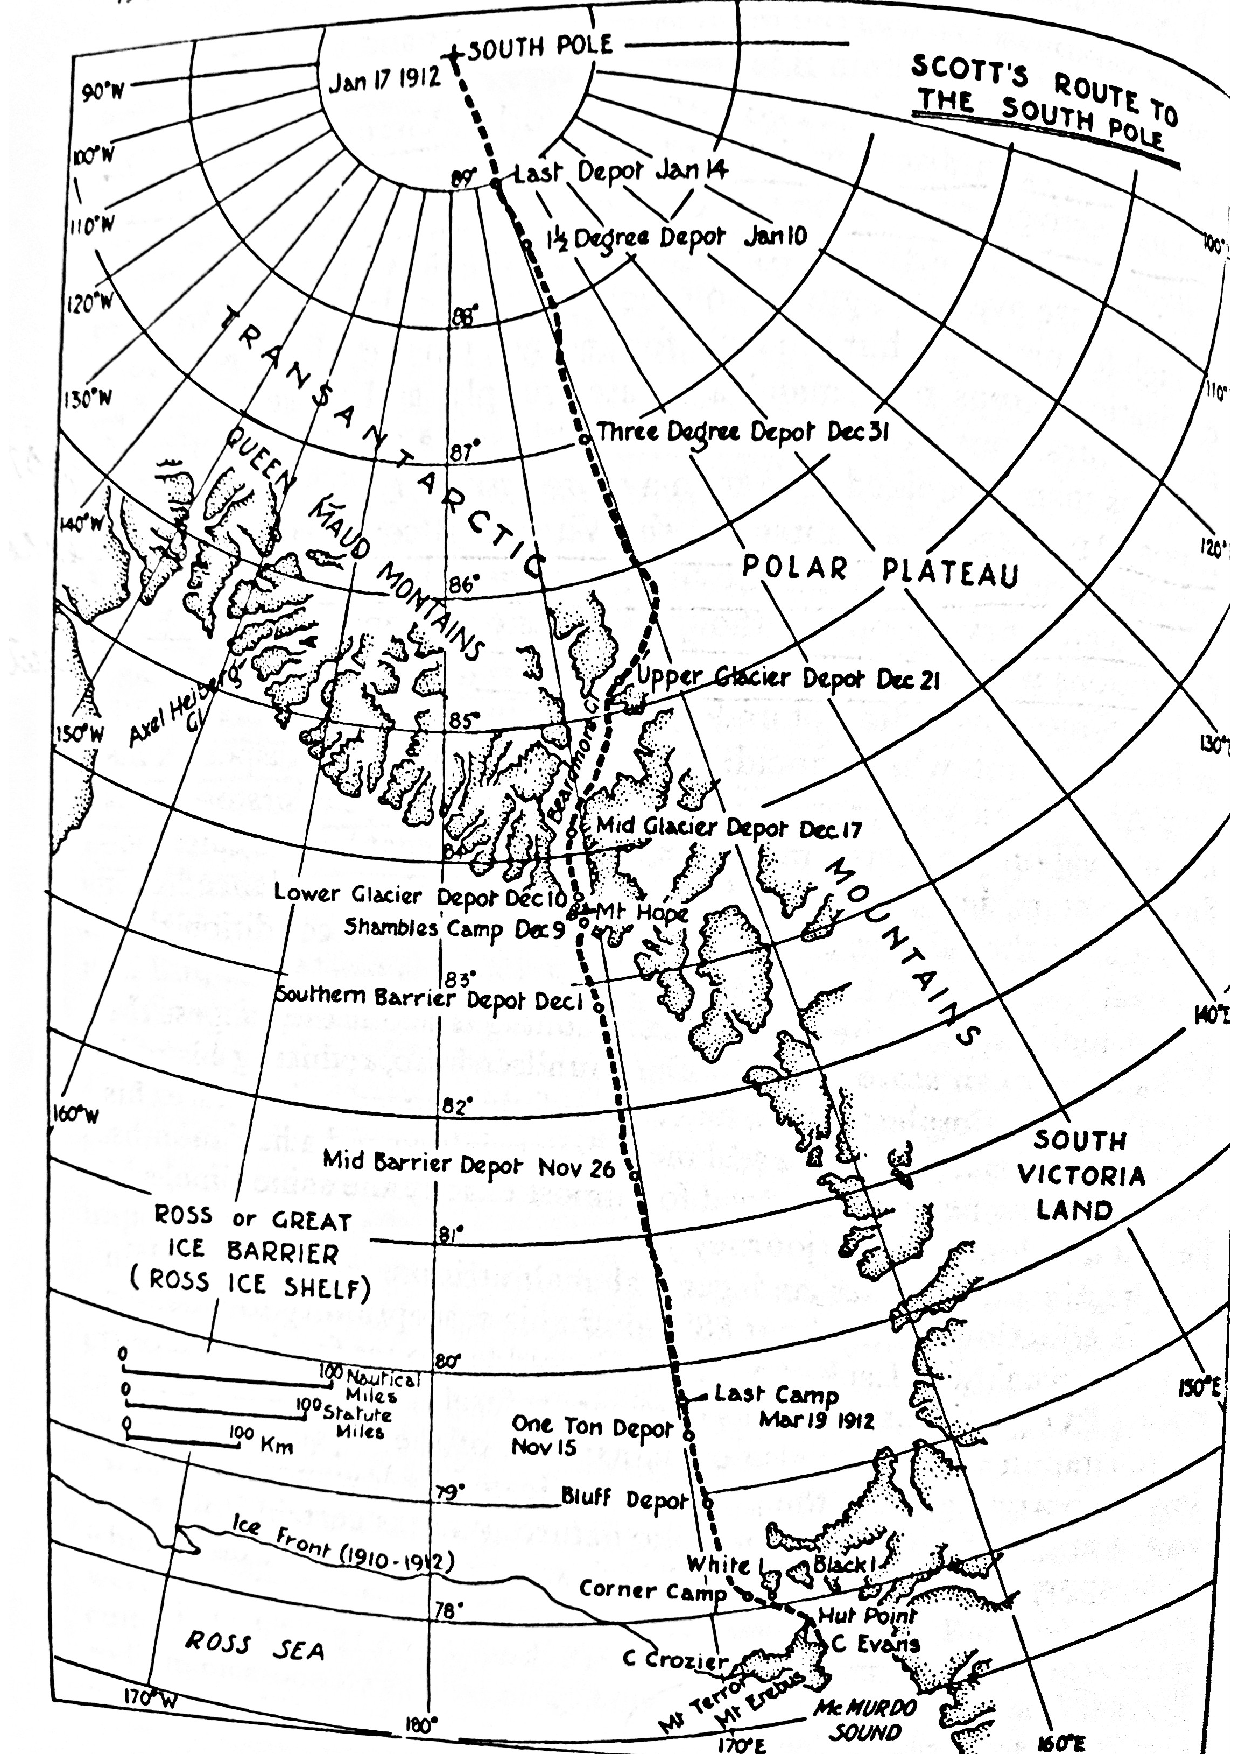
\includegraphics[width=0.3\textwidth]{scott.pdf}
\caption{\label{fig:scott} The path of Scott back to Cape Evans and Hut Point.}
\end{figure}
\end{enumerate}

\section{Chapter 32 - Back to the Fram}
\begin{enumerate}
\item How did Roald Amundsen approach base?  Do you remember how they decided to greet their three shipmates? \\ \vspace{1cm}
\end{enumerate}

\section{Chapter 3 of Deep Survival}

\begin{enumerate}
\item In chapter 3, the author describes Army Ranger training: a series of intense drills requiring extraordinary stamina and technical skill.  However, in the very next section, a former Army Ranger drowns on a rafting trip.  What caused the accident, or, why was the former Army Ranger in a survival situation? \\ \vspace{1.5cm}
\end{enumerate}

\section{Chapter 9 of Deep Survival}
\begin{enumerate}
\item Describe how Ken Killup gets lost while hiking with his friend (as the author writes in chapter 9).  What neurological processes are in play, and what parts of the brain are responsible?  What is the significance of the phrase \textit{bending the map?}  What about bewilderment?
\end{enumerate}
\end{document}
